\documentclass[10pt,letterpaper]{article}
\renewcommand{\rmdefault}{ptm}

\usepackage[left=1in,right=1in,top=1in,bottom=1in]{geometry} 
\usepackage{amsmath}
\usepackage{amsfonts}
\usepackage{amsthm}
\usepackage{amssymb}
\usepackage{polynomial}
\usepackage{layouts}
\usepackage{enumerate}
\usepackage{syntax}
\usepackage{gensymb}
\usepackage{cancel}
\usepackage{calc}
\usepackage{enumerate}
\usepackage{xcolor}

\usepackage{minted}

\usepackage[version=0.96]{pgf}
\usepackage{tikz}
\usetikzlibrary{arrows,shapes,automata,backgrounds,petri,positioning}
\usetikzlibrary{decorations.pathmorphing}
\usetikzlibrary{decorations.shapes}
\usetikzlibrary{decorations.text}
\usetikzlibrary{decorations.fractals}
\usetikzlibrary{decorations.footprints}
\usetikzlibrary{shadows}
\usetikzlibrary{calc}
\usetikzlibrary{spy}
\usetikzlibrary{matrix}

\usepackage{tikz-qtree}

\setcounter{tocdepth}{2}
\setcounter{secnumdepth}{4}
\usepackage[bookmarksopen,bookmarksdepth=3]{hyperref}
\usepackage{titlesec}


%define new colors
\definecolor{dark-red}{rgb}{0.8,0.15,0.15}
\definecolor{dark-blue}{rgb}{0.15,0.15,0.7}
\definecolor{medium-blue}{rgb}{0,0,0.5}
\definecolor{dark-green}{rgb}{0.2,0.7,0.7}

%set up color for table of contents
\hypersetup{
    colorlinks, linkcolor={dark-green},
    citecolor={dark-blue}, urlcolor={medium-blue}
}

\usepackage{tocloft}

%preven linebreak between subsection header and its content
\titleformat{\subsection}[runin]{\normalfont\bfseries}{\thesubsection.}{2pt}{}
%\titleformat{\section}[runin]{\normalfont\bfseries\filcenter}{\thesection.}{5pt}{}


\titleformat{\section}[block]
{\normalfont\sffamily\LARGE}
{\thesection}{.2em}{\titlerule\\[.2ex]\bfseries}

%title
\title{\textbf{Math 350 - Advanced Calculus \\ Homework 5}}
\author{Chan Nguyen}

%set numwidth of section
\setlength{\cftsecnumwidth}{1.5cm} 
%make subsection numwidth different than as section
\setlength{\cftsubsecnumwidth}{3cm}
%make subsection indent the same as section
\setlength{\cftsubsecindent}{\cftsecindent} 

\newcommand{\sol}{\textbf{Solution}}

\usepackage{tikz}
\usetikzlibrary{matrix}
\usetikzlibrary{shapes,backgrounds}

\makeatletter
\newcommand{\DESCRIPTION@original@item}{}
\let\DESCRIPTION@original@item\item
\newcommand*{\DESCRIPTION@envir}{DESCRIPTION}
\newlength{\DESCRIPTION@totalleftmargin}
\newlength{\DESCRIPTION@linewidth}
\newcommand{\DESCRIPTION@makelabel}[1]{\llap{#1}}%
\newcommand{\DESCRIPTION@item}[1][]{%
  \setlength{\@totalleftmargin}%
       {\DESCRIPTION@totalleftmargin+\widthof{\textbf{#1 }}-\leftmargin}%
  \setlength{\linewidth}
       {\DESCRIPTION@linewidth-\widthof{\textbf{#1 }}+\leftmargin}%
  \par\parshape \@ne \@totalleftmargin \linewidth
  \DESCRIPTION@original@item[\textbf{#1}]%
}
\newenvironment{DESCRIPTION}
  {\list{}{\setlength{\labelwidth}{0cm}%
           \let\makelabel\DESCRIPTION@makelabel}%
   \setlength{\DESCRIPTION@totalleftmargin}{\@totalleftmargin}%
   \setlength{\DESCRIPTION@linewidth}{\linewidth}%
   \renewcommand{\item}{\ifx\@currenvir\DESCRIPTION@envir
                           \expandafter\DESCRIPTION@item
                        \else
                           \expandafter\DESCRIPTION@original@item
                        \fi}}
  {\endlist}
\makeatother

\begin{document}

\tableofcontents 
\maketitle

\setlength{\parindent}{0pt}
\setlength{\parskip}{1ex}
	\phantomsection
	\subsection*{{\color{purple}\underline{Problem 1}}}
	\addcontentsline{toc}{subsection}{\numberline{}Problem 1}
	\begin{enumerate}[(i)]
		\item $\displaystyle\lim_{n\to\infty}(\sqrt[8]{n^2 + 1} - \sqrt[8]{n^2}) = 0$
		\begin{proof}
		Let $u = \sqrt[4]{n^2 + 1}, v = \sqrt[4]{n^2}$, then the limit becomes:
	 	\begin{eqnarray*}
		\displaystyle\lim_{n\to\infty} (\sqrt{u} + \sqrt{v}) 
		= \displaystyle\lim_{n\to\infty} \dfrac{u - v}{\sqrt{u} + \sqrt{v}} 
		= \displaystyle\lim_{n\to\infty} \dfrac{\sqrt{n^2 + 1} - \sqrt{n^2}}{\sqrt[8]{n^2 + 1} + \sqrt[8]{n^2}} 
		\end{eqnarray*}
		Since we already knew $\displaystyle\lim_{n\to\infty} (\sqrt{n^2 + 1} - \sqrt{n^2}) = 0$, we must have 
		$\displaystyle\lim_{n\to\infty}(\sqrt[8]{n^2 + 1} - \sqrt[8]{n^2}) = 0$
		\end{proof}
		
		\item $\displaystyle\lim_{n\to\infty}(\sqrt[8]{n^2 + 1} - \sqrt[4]{n + 1}) = 0$
		\begin{proof}		
		We have,
		\begin{eqnarray*}
		\sqrt[8]{n^2 + 1} - \sqrt[4]{n + 1} 
		&=& \sqrt[8]{n^2 + 1} - \sqrt[8]{n^2} + \sqrt[8]{n^2} - \sqrt[4]{n + 1} \\
		&=& \underbrace{\sqrt[8]{n^2 + 1} - \sqrt[8]{n^2}}_M + \underbrace{\sqrt[4]{n} - \sqrt[4]{n + 1}}_N \\
		\end{eqnarray*}
		From part (i), we already knew that $\displaystyle\lim_{n\to\infty} M = 0$, thus it remains to show
		that $\displaystyle\lim_{n\to\infty}N = 0$. Again, we can use the same technique from part (i) by 
		letting $u = \sqrt{n}, v = \sqrt{n + 1}$ to obtain,
		$$\displaystyle\lim_{n\to\infty} \dfrac{u - v}{\sqrt{u} + \sqrt{v}} = 
		\displaystyle\lim_{n\to\infty} \dfrac{n - (n + 1)}{\sqrt[4]{n} + \sqrt[4]{n + 1}}
		= \displaystyle\lim_{n\to\infty} \dfrac{-1}{{\sqrt[4]{n} + \sqrt[4]{n + 1}}}
		$$
		Apply Sandwich's lemma to 
		$$\dfrac{1}{n + n + 1} \leq \dfrac{-1}{{\sqrt[4]{n} + \sqrt[4]{n + 1}}} \leq \dfrac{-1}{\sqrt[4]{n}}$$
		we then have $\displaystyle\lim_{n\to\infty}(\sqrt[8]{n^2 + 1} - \sqrt[4]{n + 1}) = 0$
		\end{proof}
	\end{enumerate}
	
	\phantomsection
	\subsection*{{\color{purple}\underline{Problem 2}}}
	\addcontentsline{toc}{subsection}{\numberline{}Problem 2}
	Prove that if $a, b \geq 0$ then $\displaystyle\lim_{n\to\infty}\sqrt[n]{a^n + b^n} = \max(a, b)$ 
	\begin{proof} Without loss of generality, assume $\max(a, b) = a$. Since $a, b \geq 0$, we 
	have that:
	\begin{eqnarray*}
	& & \sqrt[n]{a^n} \leq \sqrt[n]{a^n + b^n} \leq \sqrt[n]{2a^n} \\
	&\Leftrightarrow & a \leq \sqrt[n]{a^n + b^n} \leq \sqrt[n]{2}a \\
	\end{eqnarray*}
	where $\displaystyle\lim_{n\to\infty} a = a$ and $\displaystyle\lim_{n\to\infty} \sqrt[n]{2} = 1$ (from homework 4).
	Apply "Algebra's of Limits" Theorem, 
	$$\displaystyle\lim_{n\to\infty} (\sqrt[n]{2} \cdot a) = 
	\displaystyle\lim_{n\to\infty} \sqrt[n]{2} \cdot \displaystyle\lim_{n\to\infty} a = 1 \cdot a = a$$  
	By Sandwich's Lemma, we must have
	$$\displaystyle\lim_{n\to\infty}\sqrt[n]{a^n + b^n} = a = \max(a, b)$$
	
	\end{proof}		
	
	
	\phantomsection
	\subsection*{{\color{purple}\underline{Problem 3}}}
	\addcontentsline{toc}{subsection}{\numberline{}Problem 3}
	\begin{enumerate}[(i)]
		\item If $r_n = \dfrac{a_{n+1}}{a_n}$, then prove that $r_{n+1} = 1 + \dfrac{1}{r_n}$
		\begin{proof}		
		Consider $r_{n+1} = \dfrac{a_{n+2}}{a_{n+1}} 
		= \dfrac{a_{n+1} + a_{n}}{a_{n+1}}
		= 1 + \dfrac{a_{n}}{a_{n+1}}
		= 1 + \dfrac{1}{r_n}$
		\end{proof}
		
		\item Let $(a_n)$ be the Fibonacci sequence, $a_0 = a_1 = 1, a_{n+2} = a_n + a_{n+1}$. 
		\begin{proof}
		To have a better understanding of the sequence $(r_n)$, we can write a quick program
		in C++, \\
\begin{minted}{c++}
#include <iostream>
#include <vector>
#include <algorithm>

using namespace std;

void fibonacci_ratio(int N) {
	int a0 = 1;
	int a1 = 1;
	int a2 = a0 + a1;
	for (int i = 0; i < N; ++i) {
		a2 = a0 + a1;
		cout << i << " : " << static_cast<double>(a2)/(a1) << endl;
		a0 = a1;
		a1 = a2;
	}
}

int main() {
	fibonacci_ratio(20);	
	return 0;
}
\end{minted} 
The outputs are: \\
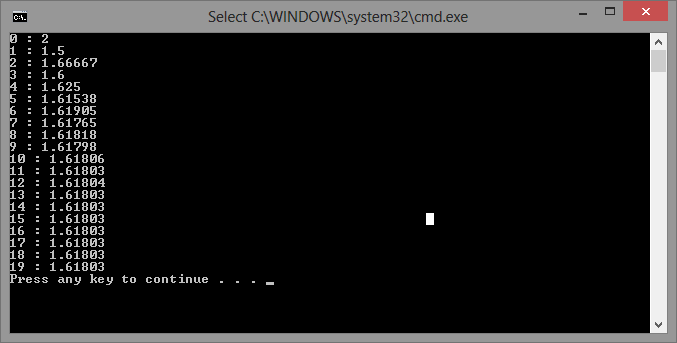
\includegraphics[scale=0.5]{hw5.png} \\
		As we can see the the even terms are decreasing and the odd terms are increasing, but both
		of them converges to $1.61803$. To prove that this sequence is converge, we first prove
		that it's bounded by $2$, then we prove that one subsequence is decreasing, the other is
		increasing. Apply Monotone Theorem, we can conclude that the sequence converges. \\
		First we prove that $r_n \leq 2$ for all $n$. We have $a_{n-1} \leq a_{n}$ for all $n$,
		hence $a_{n-1} + a_{n} \leq a_{n} + a_{n} \Leftrightarrow a_n \leq 2a_{n}$. Thus
			$$r_n = \dfrac{a_{n+1}}{a_n} \leq \dfrac{2a_n}{a_n} = 2$$
		Next we will show that $r_{n} \leq r_{n+2}$ and $r_{n+1} \geq r_{n+3}$ by induction on $n$.
		For base cases, we have:
		$$r_0 = \dfrac{a_1}{a_0} = 1, r_1 = \dfrac{a_2}{a_1} = 2, r_2 = \dfrac{a_3}{a_2} = \dfrac{3}{2}, r_3 = \dfrac{a_4}{a_3}
		= \dfrac{5}{3}$$
		So $r_0 < r_2$ and $r_1 > r_3$ are true. Now suppose that $r_{n} \leq r_{n+2}$ and $r_{n+1} \geq r_{n+3}$, we have
		$$r_{n+2} = 1 + \dfrac{1}{r_{n+1}} \leq 1 + \dfrac{1}{r_{n+3}} = r_{n+4} \text{ since } r_{n+1} \geq r_{n+3}$$
		$$r_{n+3} = 1 + \dfrac{1}{r_{n+2}} \geq 1 + \dfrac{1}{r_{n+4}} = r_{n+5} \text{ since } r_{n+2} \leq r_{n+4}$$
		Hence, we have one sequence is increasing and one sequence is decreasing, and both are bounded which implies
		they both converges. In addition, $(r_{\text{odd}}) \cup (r_{\text{even}}) = (r_n)$, so the limit exists.
		To find this limit, suppose that 
		$$\displaystyle\lim_{n\to\infty} r_n = r$$
		where $r$ is the limit that we are looking for. By property of limit, we have
		$$\displaystyle\lim_{n\to\infty} r_n = \displaystyle\lim_{n\to\infty} r_{n+1} = r$$
		In addition, from part (i) we know that $r_{n+1} = 1 + \dfrac{1}{r_n}$, so we have
		$\displaystyle\lim_{n\to\infty} r_{n+1} = \displaystyle\lim_{n\to\infty}
		\bigg(1 + \dfrac{1}{r_n}\bigg) = 1 + \displaystyle\lim_{n\to\infty}\dfrac{1}{r_n} = 
		1 + \dfrac{1}{r} = r$. So if there is solution to the equation $1 + \dfrac{1}{r} = r$, then
		the limit exists. Indeed,
		\begin{eqnarray*}
			& & 1 + \dfrac{1}{r} = r \\
			&\Leftrightarrow & r^2 - r - 1 = 0 \\
			&\Leftrightarrow & r = \dfrac{1 \pm \sqrt{5}}{2}
		\end{eqnarray*}
		On the other hand, since $a_{n} > 0$ for all $n$, $r_n = \dfrac{a_{n+1}}{a_{n}} > 0$
		which implies $r > 0$. Thus
		$$r = \dfrac{1 + \sqrt{5}}{2}$$	
		\end{proof}
	\end{enumerate}		
	
	
	
	
	
	\phantomsection
	\subsection*{{\color{purple}\underline{Problem 4}}}
	\addcontentsline{toc}{subsection}{\numberline{}Problem 4}
	Prove that the sequence $a_0, a_1, a_2 \ldots$ converges to $a$ if and only if the 
	sequence $a_0, a, a_1, a, a_2, a, a_3, \ldots$ converges. 
	\begin{proof} Since this is if only if proof, we have two cases:
		\begin{itemize}
			\item $\Rightarrow$: \\
			Since $a_0, a_1, a_2, \ldots$ converges to $a$, by definition of limit,
			for every $\epsilon > 0$, $\exists N \in \mathbb{N}$ such that for all 
			$n > N$, then $|a_n - a| < \epsilon$. Now consider the sub sequence
			$$a, a, a, a, \ldots$$
			We have that $|a - a| < \epsilon, \, \, \forall \epsilon > 0$, thus
			$a, a, a, a \ldots$ also converges to $a$. But $\{a_0, a_1, a_2, a_3, \ldots\}
			\cup \{a, a, a, a, \ldots \} = \{a_0, a, a_1, a, a_2, a, a_3, \ldots\}$. Hence,
			$a_0, a, a_1, a, a_2, a, a_3, \ldots$ converges to $a$.
			
			\item $\Leftarrow$: \\
			Suppose that $\langle a_0, a, a_1, a, a_2, a, a_3, \ldots \rangle$ converges to $L$, 
			$L \neq \pm \infty$, by definition of limit, for every $\epsilon > 0$, $\exists N \in \mathbb{N}$ 
			such that for all $n > N$, then $|a_n - L| < \epsilon$, thus there must be a sequence
			$$\langle a_{N+1}, a, a_{N+2}, a, a_{N+3}, a, a_{N+4}, \ldots \rangle$$
			that is getting closer and closer to $L$. But there is always an alternating 
			$a$ between each $a_i$ and $a_{i+1}$, so $L = a$ otherwise $|a_n - L| < \epsilon$ would
			make no sense by the choice of $\epsilon = |a - L|$. Hence,
			$$\langle a_0, a, a_1, a, a_2, a, a_3 \ldots \rangle$$
			converges to $a$. Next we will show that $\langle a_0, a_1, a_2, \ldots \rangle$ converges
			to $a$ as well. So far we have, for every $\epsilon > 0$, there exits a $N \in \mathbb{N}$
			such that for all $n > N$, $|a_n - a| < \epsilon$.
		\end{itemize}
	\end{proof}
	\textbf{Alternative proof} 
	\begin{proof}
		Choosing $N$ wisely, we actually can prove it much easier.
		\begin{itemize}
			\item $\Rightarrow$: \\
			Since $\langle a_0, a_1, a_2, \ldots \rangle$ converges to $a$, by definition of limit,
			for every $\epsilon > 0$, $\exists N \in \mathbb{N}$ such that for all 
			$n > N$, then $|a_n - a| < \epsilon$. Now consider the sequence,
			$$(b_n) = \langle a_0, a, a_1, a, a_2, a, a_3, \ldots \rangle$$
			For every $n > 2N + 1$, $|a_n - a| < \epsilon$, thus $(b_n)$ converges
			to $a$.
			
			\item $\Leftarrow$: \\
			Conversely, if $(b_n)$ converges, then all subsequences must converge
			to the same limit. Since $\langle a, a, a, \ldots \rangle$ converges to $a$, so does
			$\langle a_0, a_1, a_2, \ldots \rangle$.
		\end{itemize}
	\end{proof}
	\phantomsection
	\subsection*{{\color{purple}\underline{Problem 5}}}
	\addcontentsline{toc}{subsection}{\numberline{}Problem 5}
	Prove that $\displaystyle\lim_{n\to \infty}a_n = a$ then set of the numbers
	$A = \{a, a_0, a_1, a_2, \ldots \}$ is closed. 
	\begin{proof}
		Recall
		\newtheorem*{theo}{Theorem 7.1}
		\begin{theo}
			A number $a$ is a limit point of the set $S \subset \mathbf{R}$ if and only 
			there is a sequence of points $x_n \in S$ such that $x_n \neq a$ and $x_n \rightarrow a$.
		\end{theo}
		Since $\displaystyle\lim_{n\to\infty} a_n = a$, there exists a subsequence
		$b_{i_1}, b_{i_2}, b_{i_3} \ldots$ such that $b_n \rightarrow a$ and $b_n \neq a$ which implies
		$a$ is a limit point of the set $B = \{b_{i_1}, b_{i_2}, b_{i_3} \ldots\}$. On the other hand,
		by definition of closed set, we want to show that $A' \subset A$, so the remaining part is
		to find $A'$. Since $A = B \cup C$, where $C$ are finitely many that do not lie in $B$,
		thus $C$ is either the set that contains at least one $a$ because $B$ does not contains $a$.
		Thus $A' \subset A$ which implies $A$ is closed. 
		
	\end{proof}
		
	\phantomsection
	\subsection*{{\color{purple}\underline{Problem 6}}}
	\addcontentsline{toc}{subsection}{\numberline{}Problem 6}
	Let $a_0, a_1, a_2, a_3 \ldots$ be a bounded sequence of real numbers, and let
	$$b_n = \sup\{a_n, a_{n+1}, a_{n+2}, \ldots\}$$
	\begin{enumerate}[(i)]
		\item Prove that the sequence $b_0, b_1, b_2, b_3 \ldots$ converges. The limit
		$\displaystyle\lim_{n\to\infty}b_n$ is denoted by $\displaystyle\lim_{n\to\infty}\sup(a_n)$.
		\item Find $\displaystyle\lim_{n\to\infty}\sup(a_n)$ for each of the following:
		\begin{enumerate}
		\item $a_n = \dfrac{1}{n + 1}$
		\item $a_n = (-1)^n \dfrac{1}{n + 1}$
		\item $a_n = (-1)^n \dfrac{n}{n + 1}$
		\end{enumerate}			
	\end{enumerate}
	\begin{enumerate}[(i)]
		\item 
		First note that, in general if $A < B$ then $\sup(B) \geq \sup(A)$. 
		Since $(a_n)$ is bounded, it's bounded above and below, thus the $\sup$ exists.
		Now consider $b_n = \sup\{a_n, a_{n+1}, a_{n+2} \ldots\}$, if we look at it closed enough we 
		see that it is just the least upper bound of the subsequence of $(a_n)$ starting from index $n$.
		Hence, $\{a_{n+1}, a_{n+2}, a_{n+3}, \ldots \} \subset \{a_n, a_{n+1}, a_{n+2}, a_{n+3}, \ldots \}$
		which implies $b_{n+1}$ is an upper bound for $b_{n}$, thus
			$$b_{n} \geq b_{n+1}$$
		for all $n$ which implies $(b_n)$ is a monotonic decreasing sequence. \\
		Next we will show that
		a bounded sequence and decreasing will converge. Consider the sequence $(b_n)$. Since
		$(a_n)$ is bounded, we must have $(b_n)$ bounded because $b_n$ contains all least
		upper bounds of $(a_n)$. Thus the $b = \inf{(b_n)}$ exists. On the other hand, for all $\epsilon > 0$,
		$b + \epsilon > b$, so $b + \epsilon$ is not a lower bound for $(b_n)$. Therefore there exists
		$N \in \mathbf{N}$ such that for all $n > N$, $b_n < b + \epsilon$. Also, since $(b_n)$ is a decreasing
		sequence, $b_{n+1} \leq b_{n}$ for all $n$ which implies
		$$b - \epsilon < b \leq b_N \leq b_n < b + \epsilon
		\Leftrightarrow |b_n - b| < \epsilon \, \, \, ,\forall n > N		
		$$
		and this is precisely the definition of limit. Therefore $(b_n)$ converges.
		
		\item 
		\begin{enumerate}
		\item $a_n = \dfrac{1}{n + 1}$ \\
		As we can see, the limit of $(a_n)$ is $0$ as $n \rightarrow 0$. So the larger the index $n$,
		the closer the $sup$ to 0. In fact, for a sequence starting from index $n+1$:
			$$\{a_{n+1}, a_{n+2}, a_{n+3}, \ldots \}$$
		have the least upper bound is the first term of the sequence $a_{n}$ because $\dfrac{1}{n+1} \geq \dfrac{1}{n+2} \geq \dfrac{1}{n+3} \geq \ldots$.		
		Hence, in this case:
		$$\displaystyle\lim_{n\to\infty} \sup(a_n) = \displaystyle\lim_{n\to\infty} a_n = 0$$ 	 
		
		\item $a_n = (-1)^n \dfrac{1}{n + 1}$ \\
		This problem is slightly different from part (a) because of $(-1)^n$ which makes $(a_n)$
		alternate between negative and positive. 
		$$(a_n) = \bigg\{1, \dfrac{-1}{2}, \dfrac{1}{3}, \dfrac{-1}{4}, \dfrac{1}{5}, \dfrac{-1}{6}, 
		\dfrac{1}{7}, \dfrac{-1}{8},		
		\ldots 
		\bigg\}$$
		Look at this sequence, we can see that the least upper bound of a subsequence is no longer
		the first element because it could be a negative term. However the idea remains the same,
		suppose that we start from index 3:
		$$\bigg\{ \dfrac{-1}{4}, \dfrac{1}{5}, \dfrac{-1}{6}, 
		\dfrac{1}{7}, \dfrac{-1}{8}, \ldots \bigg\}$$
		then the $sup = \dfrac{1}{5}$. In addition, as we move further and further, the $sup$
		is getting smaller and smaller. In fact, it has the same limit as part (i), i.e.
		$$\displaystyle\lim_{n\to\infty} \sup(a_n) = \displaystyle\lim_{n\to\infty} a_n = 0$$ 	 
		
		\item $a_n = (-1)^n \dfrac{n}{n + 1}$ \\
		Let's ignore the $(-1)^n$ for a moment, and try to evaluate this limit. We have,
		$$
		\displaystyle\lim_{n\to\infty} \dfrac{n}{n + 1} = 
		\displaystyle\lim_{n\to\infty} \bigg(\dfrac{1}{1 + 1/n} \bigg) = 1
		$$
		Hence, $(a_n)$ is alternating between $-1$ and $1$. In addition, 
		$(a_n)$ is increasing because 
		$$\dfrac{n}{n+1} \leq \dfrac{n + 1}{n + 2} 
		\Leftrightarrow
		(n + 1)^2 - n(n + 2) = n^2 + 2n + 1 - n^2 - 2n = 1 > 0		
		$$
		Thus $a_n \leq a_{n+1}$ for all $n$, where $a_{n} \rightarrow 1$ so we can 
		show the sup of $(a_n)$ is 1. First we show that $1$ is an upper bound for non-empty
		set $S = (a_n)$. Since $n < n + 1 \Rightarrow \dfrac{n}{n + 1} < 1$ for all $n$. 
		Hence $1$ is an upper bound for $(a_n)$. Now suppose that there exists another 
		upper bound $u = \dfrac{1}{n + 1}$ for some integers $n$ that is smaller than $1$. 
		But $\dfrac{1}{n + 1} < \dfrac{n}{n + 1}$ which is a contradiction. Therefore
		$\sup(a_n) = 1$. From part (i), we already show that $b_n$ is a monotonic decreasing
		sequence and it converges. On the other hand since $1$ is the least upper bound for $(a_n)$, 
		it is also the least upper bound for $(a_{n+1})$ because it is decreasing. Therefore
		$$\displaystyle\lim_{n\to\infty} \sup(b_n) = 1$$
		\end{enumerate}
	\end{enumerate}
		
	\phantomsection
	\subsection*{{\color{purple}\underline{Problem 7}}}
	\addcontentsline{toc}{subsection}{\numberline{}Problem 7}
	Find all the limit points of the set $S = \{\dfrac{1}{n} + \dfrac{1}{m} : m, n \in \mathbf{N+}\}$ \\
	\begin{proof}
	First if both $m, n \rightarrow \infty$, we can prove that $0$ is one limit point.
	Recall the definition of limit point:
	\newtheorem*{tm}{Definition} 
	\begin{tm}
	A number $a$ is a limit point of a set $S \subset \mathbf{R} $ if for every $\epsilon > 0$ there is $x \in S$ such that $0 < |a - x| < \epsilon$, that is the set $S \cap (a - \epsilon, a + \epsilon) \setminus \{a\}$ is not empty.
	\end{tm}
	To show that $0$ is a limit point we can choose $N = \max(m, n)$, and for all
	$\epsilon > 0$, we have $|0 - (1/N + 1/N)| < \epsilon$. Thus $0$ is a limit point.
	Now if we fix $m$ and increase $n$, we will show that $\dfrac{1}{m}$ is also a fix point.
	Consider the set:
	$$S_1 = \{1/m + 1/n: n \in \mathbf{N}\}$$
	then for all $\epsilon > 0$, $S_1 \cap (1/m - \epsilon, 1/m + \epsilon) \setminus \{1/m\} \neq \emptyset$.
	Thus $\dfrac{1}{m}$ is also a limit point. In fact, without loss of generality, we can fix either
	$m$ or $n$ and let the other approaches $\infty$. Therefore, all limits points are:
	$$S' = \{0, \dfrac{1}{n} \mid n \in \mathbf{Z+} \}$$ 
	\end{proof}
	
	\phantomsection
	\subsection*{{\color{purple}\underline{Problem 8}}}
	\addcontentsline{toc}{subsection}{\numberline{}Problem 8}
	Let $(a_n)$ be a sequence of numbers that is bounded and injective, that is $a_n \neq a_m$ if
	$n \neq m$.
	\begin{enumerate}[(i)]
		\item Prove that if $a$ is the only limit point of the set $A = \{a_n \mid n \in \mathbf{N}\}$, then
		the sequence $a_n$ converges and $\displaystyle\lim_{n\to \infty}a_n = a$.
		\begin{proof}
		Since $a$ is the only limit point of $A = \{a_n \mid n \in \mathbf{N}\}$, by Theorem 7.1, 
		there exists a sequence points $a_n \in A$ such that $a_n \neq a$ and $a_n \rightarrow a$. 
		Also from the definition of limit point, there exists a $\epsilon > 0$, such that the interval
		$(a - \epsilon, a + \epsilon)$ contains all $a_n \in A$, except for some finite terms that are
		not in this interval. Let denote this outside sequence as 
		$$(b_n) = \{b_{i_1}, b_{i_2}, b_{i_3}, \ldots, b_{i_k}\}$$
		Note that we can't assume the index is from $1 \rightarrow k$, because it's not necessary
		for there terms to be in a particular order. In other words, the index could be arbitrary
		as long as $b_n \in A$, and $b_n \not\in (a - \epsilon, a + \epsilon)$. Furthermore,
		since $a$ is the only limit point, there must be only two types of sequence, either $\in 
		(a - \epsilon, a + \epsilon)$ or $\not\in (a - \epsilon, a + \epsilon)$.
		Next
		let's $N = \max(i_1, i_2, i_3, \ldots, i_k)$
		then $N + 1$ must be in $(l - \epsilon, l + \epsilon)$. Hence for all $n \geq N + 1$
		$a_n \in (a - \epsilon, a + \epsilon)$ which implies for all $\epsilon > 0$, there exists
		$N + 1 = M \in \mathbf{N}$ such that $|a_n - a| < \epsilon$ for all $n \geq M$ which is 
		precisely the definition of limit. Therefore $\displaystyle\lim_{n\to\infty} a_n = a$.	
		\end{proof}
		Another way to prove it,
		\begin{proof}
		Suppose $a_n$ does not converges to $a$, then there is $\epsilon > 0$ such that
		for every natural number $k$, there is $n_k > k$ such that $|a_{n_k} - a| \geq \epsilon$.
		The sequence $(a_{n_k})$ is a subsequence of $(a_n)$ thus is bounded. Therefore it has 
		a subsequence $(a_{n_{kl}})$ which converges to a point $b \neq a$ because $|a_{n_{kl}} - a| > \epsilon$.
		In addition, the sequence $(a_n)$ is one-to-one, all elements of this sequence are distinct
		and therefore $b$ is a limit point of $(a_n)$. 
		\end{proof}
		
		\item Show by a counterexample that this property is not true for unbounded sequences.
		\begin{proof}
		A counter example could be
		$$\{1, 1/2, 2, 1/3, 3, 1/4, 4, 1/5, \ldots\}$$
		which have only one limit point $0$ because $\displaystyle\lim_{n\to\infty} \dfrac{1}{n} = 0$
		and the sequence of all natural number is unbounded, thus does not converge.
		\end{proof}
	\end{enumerate}
	
	\phantomsection
	\subsection*{{\color{purple}\underline{Problem 9}}}
	\addcontentsline{toc}{subsection}{\numberline{}Problem 9}
	Prove that a set $S \subset \mathbb{R}$ is bounded if and only if every sequence of points 
	in $S$ has a convergent subsequence.
	\begin{proof}
	Assume that $S \subset \mathbb{R}$ is bounded. 
	If $(x_n)$ is a sequence in $S$ , then $(x_n)$ is bounded and thus it has a convergent subsequence.
	Assume that $S$ is not bounded, then for any integer $n$ there is an $x_n$ in $S$ such that $|x_n| > n$. 
	Since any convergent sequence is bounded, the sequence $(x_n)$ cannot have a convergent subsequence.
	\end{proof}
\end{document}
